%% This paper was borne from a template by Michael Shell named bare_jrnl.tex V1.4b dated 2015/08/26

\documentclass[journal]{IEEEtran}

\usepackage{array}
\usepackage{algorithm}
\usepackage{algpseudocode}
\usepackage{amsfonts}
\usepackage{amsmath}
\usepackage{bm}
\usepackage{cite}
\usepackage{graphicx}
\usepackage{subcaption}
\usepackage[caption=false,font=normalsize,labelfont=sf,textfont=sf]{subfig}
\usepackage{float}
\usepackage{url}

% graphicx declarations
\graphicspath{{../images/}}
\DeclareGraphicsExtensions{.jpeg,.jpg,.png}
\DeclareMathOperator*{\argmin}{arg\,min}

% *** Do not adjust lengths that control margins, column widths, etc. ***
% *** Do not use packages that alter fonts (such as pslatex).         ***

% correct bad hyphenation here
\hyphenation{op-tical net-works semi-conduc-tor}

\begin{document}
\title{Review of Linear Spectral Mixture Analysis}

\author{Bernard~Lampe,~\IEEEmembership{Student Member,~IEEE}}

% The paper headers
\markboth{Review of Linear Spectral Mixture Analysis Algorithm}
{Lampe \MakeLowercase{\textit{et al.}}: Review of Linear Spectral Mixture Analysis Algorithms}

% make the title area
\maketitle

% As a general rule, do not put math, special symbols or citations in the abstract or keywords.
\begin{abstract}
Linear spectral mixture analysis (LSMA) is a ubiquitous theory applied to hyperspectral images (HSI) to determine the presence and quantity of known materials by decomposing the pixels into parts. The analysis can be performed in a supervised or unsupervised manner. In the supervised case, the model assumes the pixels are each linearly mixed from a set of known spectral signatures. In the unsupervised case, the analysis must find the number of spectral signatures and the signatures themselves as well as decompose each pixel into a linear combination of those found signatures. The methods of finding the spectral signatures are referred to as HSI unmixing.  In this study, we review, implement and test five supervised LSMA algorithms to unmix hyperspectral pixel vectors into parts. The purpose of this review is to understand the differences in the algorithm approaches to solving LSMA and the positives and drawbacks of using the algorithms. The accuracy and algorithm timing are then used to numerically evaluate the algorithms.
\end{abstract}

\begin{IEEEkeywords}
Hyperspectral, Linear Spectral Mixture Analysis (LSMA), Active Set Methods, Geometric Method, Orthogonal Subspace Projection, Fully-Constrained-Least-Squares (FCLS), Modified FCLS
\end{IEEEkeywords}

\section{Introduction}
\IEEEPARstart{L}{inear} spectral mixture analysis (LSMA) takes advantage of the linear mixture model (LMM) and assumes that all the hyperspectral pixels can be represented as a constrained linear combination of vectors \cite{changbook1}. LSMA postulated that any HSI image of \(L\) bands is a linear combinations of a finite set of \(p\) pure signatures \(\mathbf{t}_1, \mathbf{t}_2, ..., \mathbf{t}_p\) where \(\mathbf{t}\) is a \(Lx1\) vector. These pure signatures are quantized and measured and the resulting spectral signatures of dimension \(Lx1\) are \(\mathbf{m}_1, \mathbf{m}_2, ...\mathbf{m}_p\). The linear mixture model then further states that each HSI pixel vector \(\mathbf{r}_i\) for \(i=1\) to \(N\) image pixels is a linear combination of the spectral signatures as denoted in equation \ref{eq:lmm}. This model arranges the spectral signatures into a matrix \(\mathbf{M}\) and the goal of supervised LSMA is to find the \(p\) constrained abundance fractions in \(\mathbf{\alpha}_i\). In order to have a model that is consistent with real hyperspectral images, the abundance fractions are constrained to sum-to-one (ASC) and to be non-negative (ANC). The model also includes an error term \(\mathbf{n}\) to account for model error, measurement error, noise and background.

There are two critical questions which must be resolved when using the linear mixture model for LSMA \cite{changbook3}. The first is how to estimate the number of spectral signatures will be required \(p\). This parameter must be chosen with care to ensure that the model is sufficient and efficient. The second is how to determine the constrained abundance fractions. The abundance fractions are constrained to sum-to-one (ASC) and to be non-negative (ANC). In supervised LSMA, we are given the \(\mathbf{M}\) matrix and \(p\). In this study, we review five supervised algorithms. The unsupervised unmixing problem is harder and we use non-negative matrix factorization (NMF) to determine \(\mathbf{M}\) and \(\mathbf{\alpha}_i\) simultaneously.

An interesting point of the LSMA algorithms is the way they view the LMM when deriving the algorithms. Each model assumes the pixels are a combination of the spectral signatures, but they vary in the way they assign a pixel to those signatures. We have noted three popular interpretations of the model. The first is the spectral components based model. This model is most popular and best represented by equation \ref{eq:lmm} where the pixel \(\mathbf{r}_i\) is an affine linear combination of non-negative abundance fractions. The second interpretation of the model is based on clustering algorithms. The set of spectral signatures \(\left\{\mathbf{m}_i\right\}_{i=1}^p\) are the cluster centers and the abundance fractions are the cluster assignments. Each pixel is then given an assignment value representing the clusters contribution to the pixel. The last noted understanding of the LMM is the simplex model. In this view the spectral signatures represent the vertices of a simplex. Then the abundance fractions represent the location of pixel vector inside the simplex. Each of these understandings of the model lead to unique algorithms for LSMA which will be relevant for our review.

\begin{equation}
\label{eq:lmm}
\mathbf{r}_i = \mathbf{M}\mathbf{\alpha}_i + \mathbf{n}
\end{equation}

\section{Fully Constrained Linear Spectral Mixture Analysis Results}
In this section we will review three FCLS algorithms for determining the constrained abundance fractions. Each algorithm will compute the abundance fractions given the spectral signatures \(\mathbf{M}\). Each algorithm incorporates the sum-to-one constraint (ASC) and the non-negativity constraint (ANC) in different ways.

\subsection{Active Set Method}
The active set method developed by Heinz and Chang can be used to solve the FCLS as an iterative algorithm which is initialized by the unconstrained least squares solution \(\mathbf{\alpha}_i^{LS} = \left(\mathbf{M}^T\mathbf{M}\right)^{-1}\mathbf{M}^T\mathbf{r}_i\) \cite{heinz}. The optimization utilizes the non-negative least squares constrained (NCLS) algorithm to refine the initial solution. The iteration begins by making two sets which track the passive and active components of the optimization. The unconstrained least squares solution can have negative values which violate the model. Those dimensions of the model become active while the remaining are passive. The active dimensions are used to perform a gradient descent until the negative components become non-negative. In order to impose the sum-to-one constraint (ASC), the spectral signature matrix and pixel are augmented to include a unitary dimension as in equation \ref{eq:asc}. This dimension enforces the ASC approximately by down weighting the other dimension values by using \(\delta = 1/max{(m_{ij})}\). The vectors \(\mathbf{\tilde{r}}\) and the matrix \(\mathbf{\tilde{M}}\) take the place of \(\mathbf{r}\) and \(\mathbf{M}\) during the optimization.

\begin{equation}
\label{eq:asc}
\mathbf{\tilde{r}} = \begin{bmatrix}
\delta\mathbf{r} \\ 1
\end{bmatrix},
\mathbf{\tilde{M}} = \begin{bmatrix}
\delta \mathbf{M} \\ \mathbf{1}^T
\end{bmatrix}
\end{equation}

\subsection{Geometric Method}
The geometric method for solving FCLS was put forth by Wang, Liu and Wang \cite{liguo}. This method is a close form solution which takes advantage of Cramer's rule from calculus. This rule states that the solution of a critically determined linear system can be solved one component at a time using the ratio of determinants. The FCLS algorithm can take advantage of this by noting the determinant is the volume of the simplex formed by the vertices of the spectral signatures \(\left\{\mathbf{m}_i\right\}_{i=1}^p\).

The algorithm proceeds by introducing the unitary dimension just as the active set method did in order to impose the ASC as in equation \ref{eq:gasc}. Then the computation of the volume for each simplex is then performed to compute the abundance fractions as in equation \ref{eq:gvol}.

\begin{equation}
\label{eq:gasc}
\mathbf{\tilde{r}} = \begin{bmatrix}
1 \\ \mathbf{r}
\end{bmatrix},
\mathbf{\tilde{M}} =
\begin{bmatrix}
1 & 1 & ... & 1 \\
\mathbf{m}_1 & \mathbf{m}_2 & ... & \mathbf{m}_p
\end{bmatrix}
\end{equation}

The determinant of the matrix \(\mathbf{\tilde{M}}\) is not defined because it is not square. Some algorithms perform PCA to project to a lower dimension to compute the projected volume. However, this algorithm computes the volume using equation \ref{eq:gvol}.

\begin{equation}
\label{eq:gvol}
Vol(\mathbf{\tilde{m}}_1, \mathbf{\tilde{m}}_2, ..., \mathbf{\tilde{m}}_p) = \frac{1}{(p-1)!}\sqrt{|\mathbf{\tilde{M}}^T\mathbf{\tilde{M}}|}
\end{equation}

The abundance fraction components are computed as the ratio of the volumes of the augmented spectral signature matrix and the unmodified spectral signature matrix. The volumes are computed so the sign of the numerator and denominator are the same which ensures the non-negativity of the result.

\begin{equation}
\label{eq:gabundance}
\alpha_i = \frac{Vol(\mathbf{\tilde{m}}_1, ..., \mathbf{\tilde{m}}_{i-1}, \mathbf{\tilde{r}}, \mathbf{\tilde{m}}_{i+1}, ..., \mathbf{\tilde{m}}_p)}{Vol(\mathbf{\tilde{m}}_1, \mathbf{\tilde{m}}_2, ..., \mathbf{\tilde{m}}_p)}
\end{equation}

\subsection{OSP Method}
The last FCLS method reviewed takes advantage of the orthogonal subspace projection (OSP) projector to suppress the signatures not of interest. The projector is computed by removing the spectral signature of interest as in equation \ref{eq:osp_m}. Then computing the projector to suppress the other signatures as in equation \ref{eq:osp_p}. These \(p\) projectors are used to estimate the contribution of each signature. The magnitudes of the projections are the abundance fractions.

\begin{equation}
\label{eq:osp_m}
\mathbf{\tilde{M}} = \left[\mathbf{m}_1,...,\mathbf{m}_{i-1}, \mathbf{m}_{i+1}, ..., \mathbf{m}_p\right]
\end{equation}

\begin{equation}
\label{eq:osp_p}
\delta_{\mathbf{m}_i}=\mathbf{P}_{\mathbf{U}}^\perp = \mathbf{I} - \mathbf{\tilde{M}}\left(\mathbf{\tilde{M}}^T\mathbf{\tilde{M}}\right)^{-1}\mathbf{\tilde{M}}^T
\end{equation}

\section{Modified Fully Constrained Linear Spectral Mixture Analysis}
The modified FCLS (MFCLS) algorithm developed by Wong and Chang, makes use of two insightful constraints that allows for the Lagrange multiplier solution to be implemented \cite{wong}. The MFCLS approach takes advantage of the ASC but adds another constraint using the absolute value, abundance sum-to-one constraint (AASC) as in equation \ref{eq:aasc}. These constraints results in an algorithm which is solvable with minimal iteration via Lagrange multiplier. There are two version of the algorithm we will review.

\begin{equation}
\label{eq:aasc}
\sum_{i=1}^{p}\alpha_i = 1 \text{          and         } \sum_{i=1}^{p}|\alpha_i| = 1
\end{equation}

\subsection{Lagrange Multiplier}
The first version of the algorithm is below. Note that the algorithm is initialized by the \(\mathbf{\alpha}^{SCLS}\) which is the sum-to-one constrained abundance solution presented by Heinz and Chang \cite{heinz}. Also, note the operator \(sign(\mathbf{\alpha})\) is the vector consisting of the sign of each entry such as \(sign(\alpha_i) = \alpha_i/|\alpha_i|\).

\begin{enumerate}
\item Initial condition is \(\mathbf{\alpha}^{MFCLS}=\mathbf{\alpha}^{SCLS}\)
\item Compute \(\lambda_1\) and \(\lambda_2\) using constraints \(\sum_{i=1}^{p}\alpha_i = 1\) and \(\sum_{i=1}^{p}|\alpha_i| = 1\)
\item \({\mathbf{\alpha}^{MFCLS}=\mathbf{\alpha}^{SCLS}-\left(\mathbf{M}^T\mathbf{M}\right)^{-1}\left[\lambda_1\mathbf{1}+\lambda_2 sign(\mathbf{\alpha}^{SCLS})\right]}\)
\item Iterate if any negative components left
\end{enumerate}

The second step of the MFCLS algorithm is to compute \(\lambda_1, \lambda_2\). These are computed using the ASC and AASC. When forming the problem, the following matrix in equations \ref{eq:mfcls_matrix1} and \ref{eq:mfcls_matrix2} are derived. This \(2x2\) linear system is readily solvable for \(\lambda_1\) and \(\lambda_2\).

\begin{equation}
\label{eq:mfcls_matrix1}
\begin{bmatrix}
1-\mathbf{1}^T\mathbf{\alpha}^{MFCLS} \\
1-sign(\mathbf{\alpha}_{LS})^T\mathbf{\alpha}^{MFCLS}
\end{bmatrix}
\mathbf{X} = \\
\begin{bmatrix}
\lambda_1 \\ \lambda_2
\end{bmatrix}
\end{equation}

\begin{equation}
\label{eq:mfcls_matrix2}
\mathbf{X} = \begin{bmatrix}
\mathbf{1}^T(\mathbf{M}^T\mathbf{M})^{-1}\mathbf{1} & \mathbf{1}^T(\mathbf{M}^T\mathbf{M})^{-1} sign(\mathbf{\alpha}_{LS}) \\
sign(\mathbf{\alpha}_{LS})^T(\mathbf{M}^T\mathbf{M})^{-1}\mathbf{1} & sign(\mathbf{\alpha}_{LS}^T) (\mathbf{M}^T\mathbf{M})^{-1} sign(\mathbf{\alpha}_{LS})
\end{bmatrix}
\end{equation}

\subsection{Iterative Algorithm}
The iterative algorithm for MFCLS put forth by Wong and Chang is similar to the active set method \cite{wong}. The algorithm chooses an active set and performs gradient descent on the dimensions chosen. However, the steering matrix computed during gradient descent is augmented to include the ASC and AASC constraints. This results in few iterations of the algorithm when compared to active set FCLS.

\begin{equation}
\mathbf{s} = \begin{bmatrix}
\delta\mathbf{r} \\ 1
\end{bmatrix},
\mathbf{N} = \begin{bmatrix}
\delta \mathbf{M} \\ \mathbf{1}^T
\end{bmatrix}
\end{equation}

\begin{equation}
\label{eq:mse}
\argmin_{\mathbf{\hat{M}},\mathbf{\hat{A}}}\left\{\|\mathbf{X} - \mathbf{\hat{M}}\mathbf{\hat{A}}\|^2\right\}
\end{equation}

\section{Hyperspectral Data}
We used the simulated data to test each of the LSMA and NMF algorithms. We did experiments on the TI2 and TE2 data sets described in Dr. Chang's book \cite{changbook2}. The data sets each take spectral signatures extracted from the Cuprite data set for five different materials. The full image with the extracted data set spatial locations are in figure \ref{fig:cuprite}. The spectral signatures are plotted in figure \ref{fig:reflectance}. The five material types are  1Alunite, Buddingtonite, Calcite, Kaolinite and Muscovite. Each spectral signature was added to the image in an intentional programmatic way to demonstrate algorithm performance. Each material is given a primary row and the first column is a \(4x4\) pure pixel panel, the second column is a \(2x2\) pure pixel panel, the third column is a \(2x2\) pixel panel where each pixel is a \(50\)\% mixture of the primary material for the row and the other four materials. The fourth column is a \(1x1\) sub-pixel signature which consists of \(50\)\% signature and \(50\)\% background. The fifth column is also a subpixel with \(25\)\% material and \(75\)\% background. Each image has a \(20\) db SNR. The TI image (target implant) is designed by removing the background pixel and inserting the pure signature pixel. The TE image (target embedded) is designed by super-imposing the pure signature and the background as a linear combination. Therefore, for a TI2 pixel, the panel pixels are described as \(\mathbf{r}_i=\mathbf{m}_i+\mathbf{n}\) and the TE2 panel pixels are described as \(\mathbf{r}_i=\mathbf{m}_i+\mathbf{b}+\mathbf{n}\) where \(\mathbf{b}\) is a background signature.

\section{Experiment Results}
The numeric experimental results are shown in Table I and Table II. The accuracy of the result was computed as the MSE of the abundance fractions of the panel pixels only. The background pixels were ignored because we do not have ground truth for them. The abundance fractions for the first two columns of panels should be \(1\) for all panel pixels. For the third and fourth columns the abundance should be \(0.5\) and the fifth column should be \(0.25\). You can see from Table I that the accuracy for the TI2 image is much better overall than the TE2. The accuracy of TI2 is much higher because the spectral signatures implanted in the image where not corrupted by background. Another way of seeing why this is the case is that the pixels of TI2 are within the simplex volume of the spectral signatures used in FCLS in \(\mathbf{M}\). Within the simplex volume the matrix \(\mathbf{M}^T\mathbf{M}\) used for gradient descent is convex. However outside the simplex volume the problem may not be convex and could diverge when doing gradient descent. This occurs in the TE2 case where the pixels are added to a background pixel which is not accounted for in the spectral signature matrix \(\mathbf{M}\).

Another observation is that the active set and modified FCLS algorithms worked best overall. These algorithms are initialized with the \(\mathbf{\alpha}^{LS}\) and the \(\mathbf{\alpha}^{SCLS}\) solutions which are close to the optimum. Then the final solutions are computed using the gradient via gradient descent or Lagrange multiplier.

\begin{table}[!h]
    \caption{Algorithm accuracy in MSE, a. Active Set FCLS b. Geometric FCLS c. OSP FCLS d. MFCLS Lagrange e.MFCLS Iterative}
    \centering
    \begin{tabular}{|c|c|c|c|c|c|}
    \hline
        & A. & B. & C. & D. & E. \\ \hline
    TI2 & 0.003489& 0.00394& 0.01672& 0.003536& 0.003538\\ \hline
    TE2 & 0.709771& 0.13506& 0.02976& 5.677302& 143345.3 \\ \hline
    \end{tabular}
\end{table}

We evaluated the algorithm run times and found that the geometric algorithm is fastest overall while the iterative MFCLS is comparably slow.

\begin{table}[!h]
    \caption{Algorithm timing in seconds, a. Active Set FCLS b. Geometric FCLS c. OSP FCLS d. MFCLS Lagrange e. MFCLS Iterative}
    \centering
    \begin{tabular}{|c|c|c|c|c|c|}
    \hline
    3.263822& 1.762295& 1.880125&  2.453860& 9.055446 \\
    \hline
    \end{tabular}
\end{table}

The abundance fractions for all FCLS algorithms on TI2 data are displayed in figures 4 to 8. The results are much more accurate when compared to the TE2 results in figures 9 through 13. However, in the TE2 case the OSP algorithm did much better than all other algorithms on TE2. This is because the algorithm suppresses the other spectral signatures without modifying the primary signature.

The results for the direct NMF algorithm are in figures 14 to 17. While this algorithm was initialized with the spectral signatures matrix \(\mathbf{M}\), the results are not impressive. The algorithm quickly ends up in a bad state. We see the same effect in figures 18 to 21 for the sparse NMF algorithm.

\section{Conclusions}
The FCLS works well on the TI2 data set because the spectral signature set accounts for the panel pixels in the image. The TE2 image results are poor because the background added to the panel pixels is not accounted for in the spectral signature matrix.  The active set and modified FCLS algorithms were most accurate overall on the TI2 data set. The OSP was the best performing algorithm on the TE2 data set. Overall, the geometric algorithm was the fastest and almost as accurate as the other FCLS algorithms.

The alternating least squares and multiplicative updates methods for the non-negative matrix factorization results were poor even when enforcing sum-to-one using the augmented mixture matrix with unity dimension. Adding sparsity and incoherence to the algorithm helped and was necessary for the unsupervised method.

\begin{figure}[!h]
    \centering
    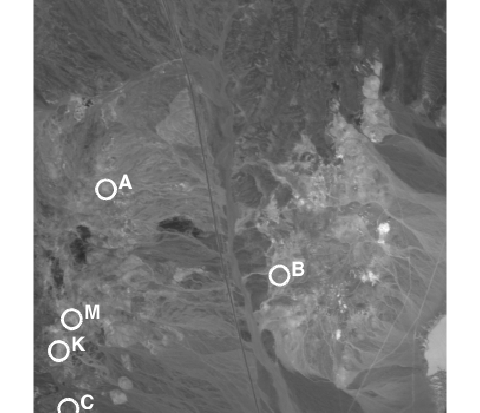
\includegraphics[width=3.20in]{cuprite_groundTruth.png}
    \caption{Cuprite Data, Band 80, Marking Materials}
    \label{fig:cuprite}
\end{figure}

\begin{figure}[!h]
    \centering
    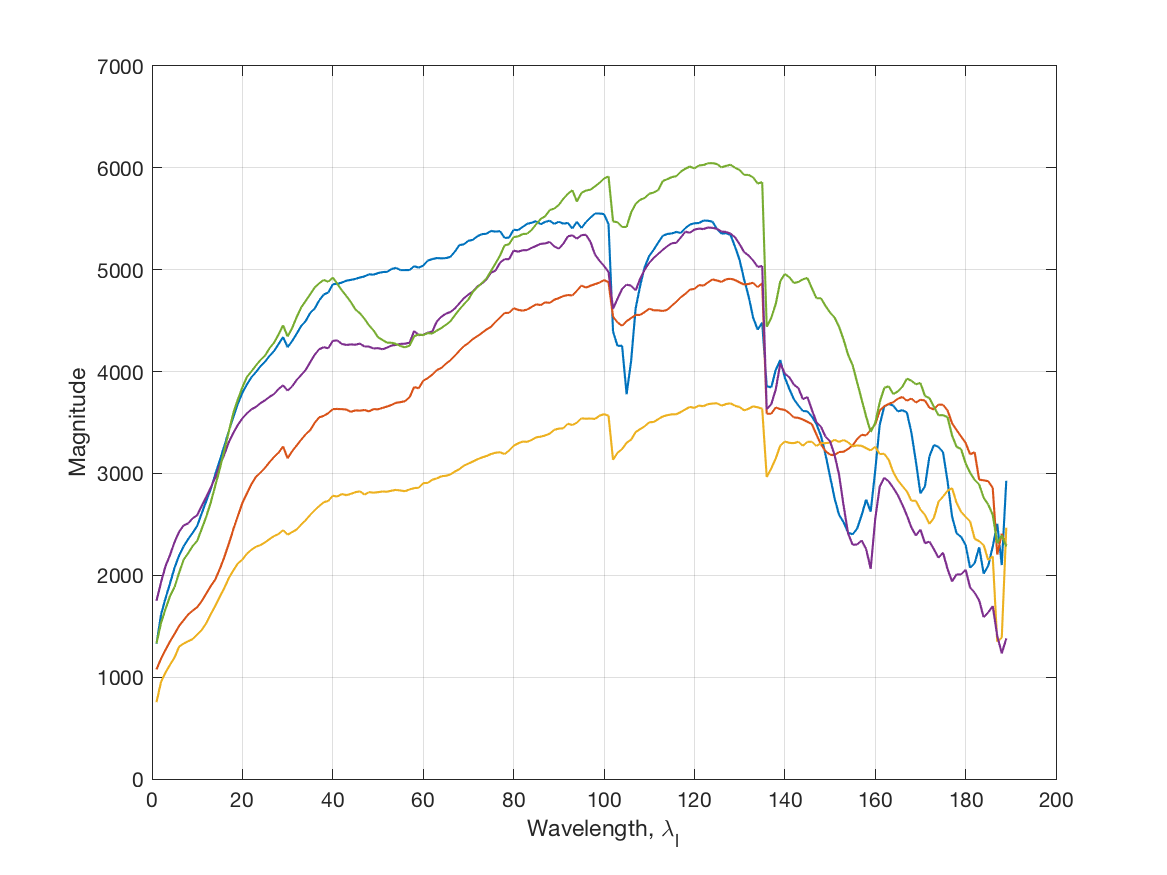
\includegraphics[width=3.20in]{reflectance.png}
    \caption{Plotted reflectance for A, B, C, K, and M materials}
    \label{fig:reflectance}
\end{figure}

\begin{figure}[!h]
    \centering
    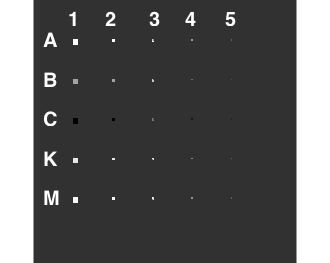
\includegraphics[width=3.5in]{synthetic_labeled.png}
    \caption{Synthetically generated data pure pixels in the Cuprite image TE2.}
    \label{fig:syn}
\end{figure}

%fcls_ti2_allmaterials.png
\begin{figure}[!h]
    \centering
    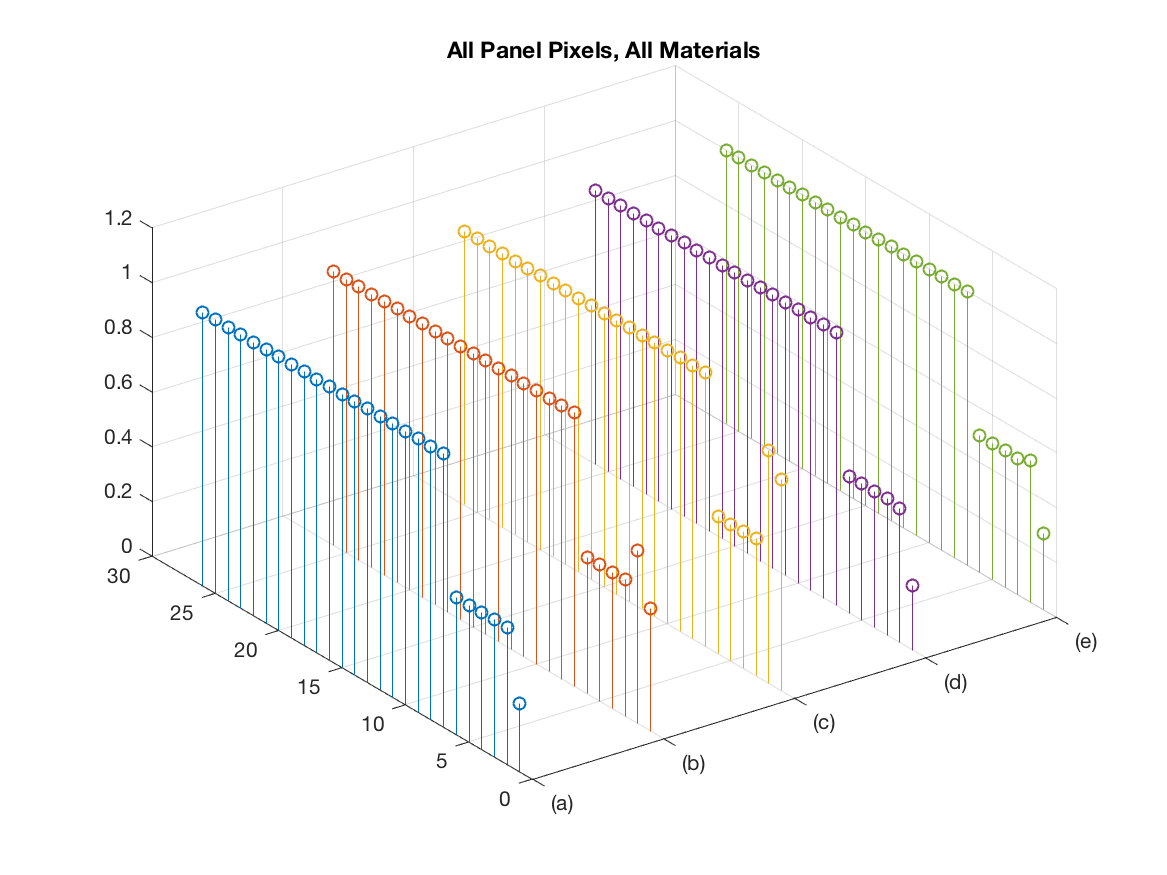
\includegraphics[width=3.5in]{fcls_ti2_allmaterials.png}
    \caption{FCLS, Active Set Method for TI2}
    \label{fig:fcls_ti2}
\end{figure}

%gfcls_ti2_allmaterials.png
\begin{figure}[!h]
    \centering
    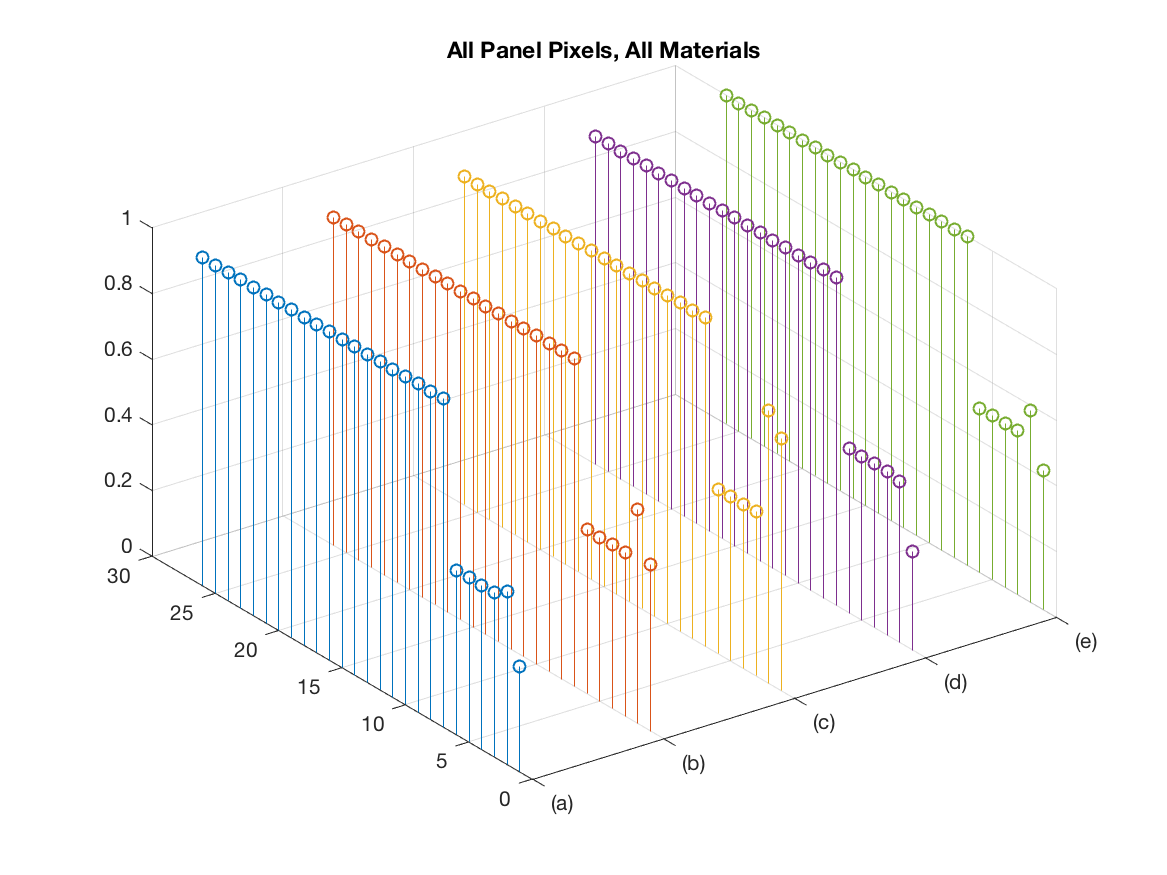
\includegraphics[width=3.5in]{gfcls_ti2_allmaterials.png}
    \caption{FCLS, Geometric Volume Method for TI2}
    \label{fig:gfcls_ti2}
\end{figure}

%osp_fcls_ti2_allmaterials.png
\begin{figure}[!h]
    \centering
    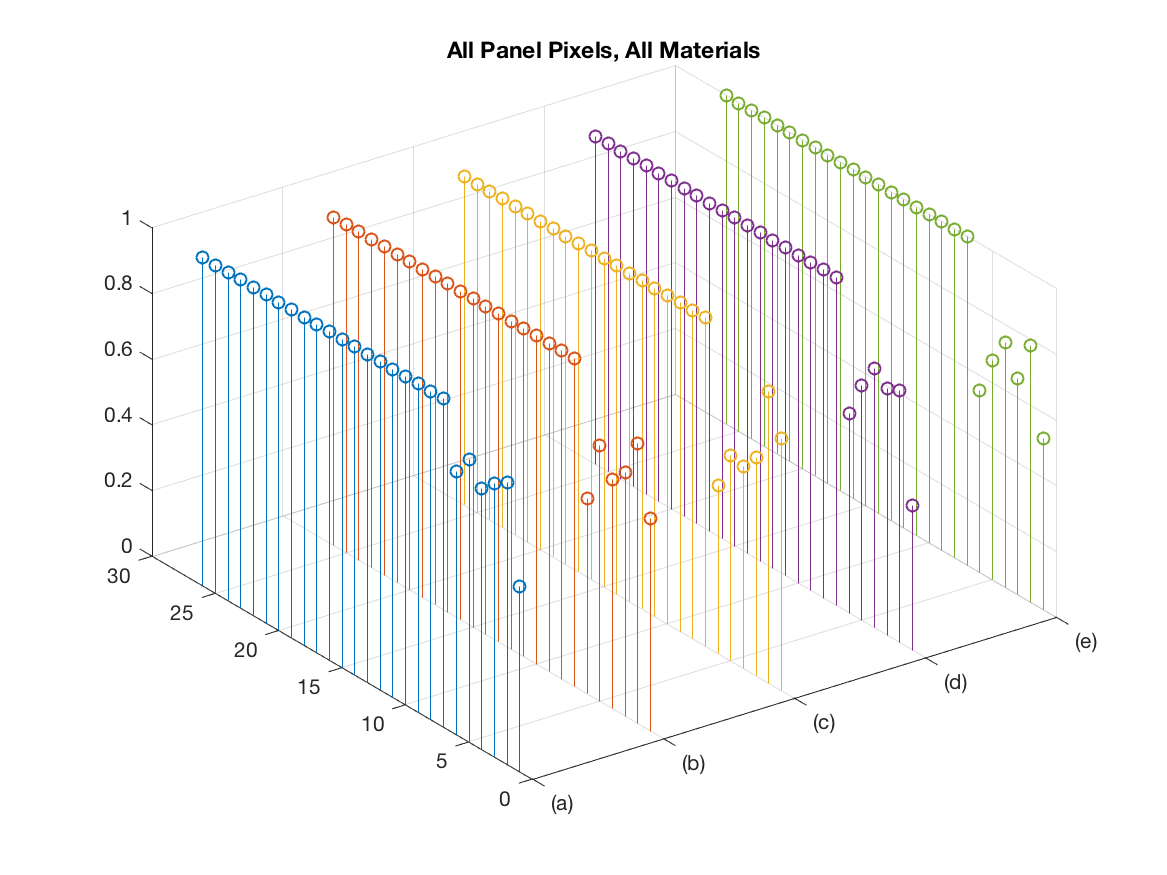
\includegraphics[width=3.5in]{osp_fcls_ti2_allmaterials.png}
    \caption{FCLS, OSP Method for TI2}
    \label{fig:osp_fcls_ti2}
\end{figure}

%mfcls2_ti2_allmaterials.png
\begin{figure}[!h]
    \centering
    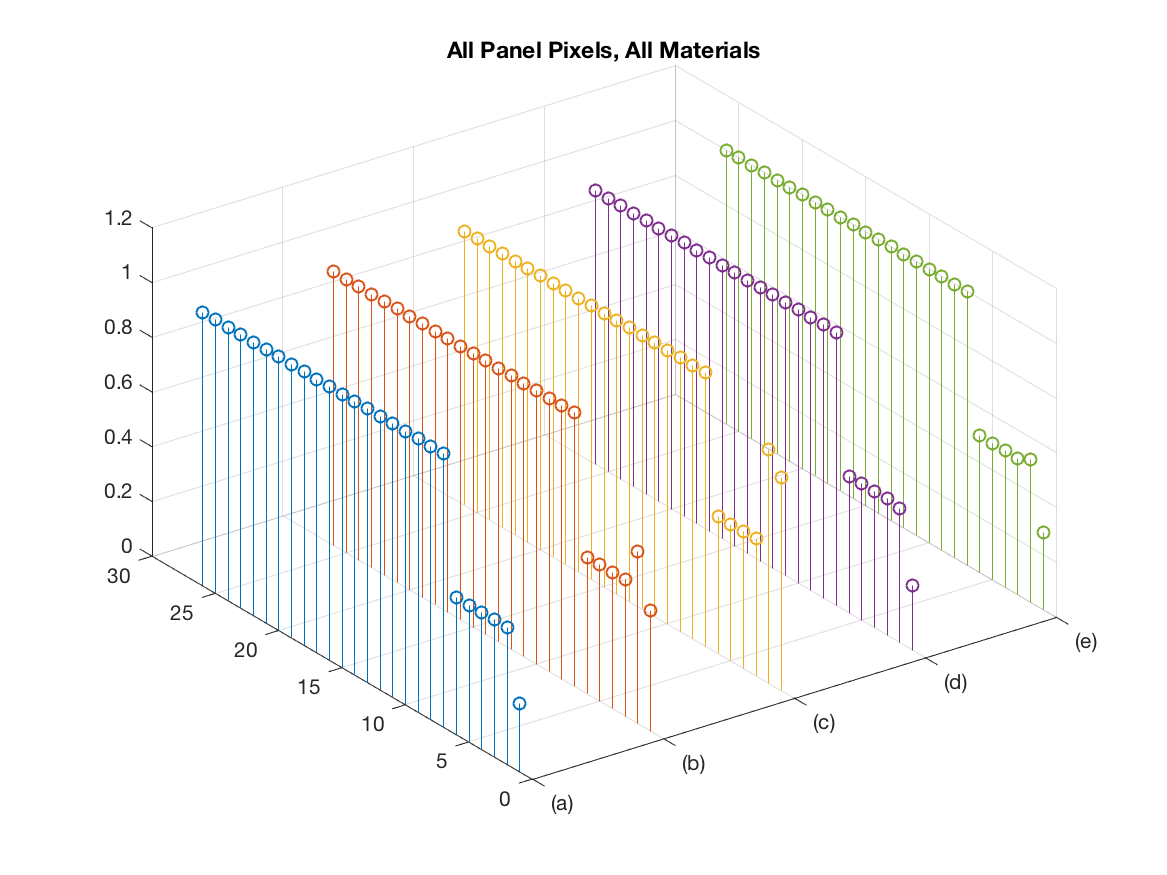
\includegraphics[width=3.5in]{mfcls2_ti2_allmaterials.png}
    \caption{MFCLS, Lagrange Multiplier Method for TI2}
    \label{fig:mfcls2_ti2}
\end{figure}

%mfcls_ti2_allmaterials.png
\begin{figure}[!h]
    \centering
    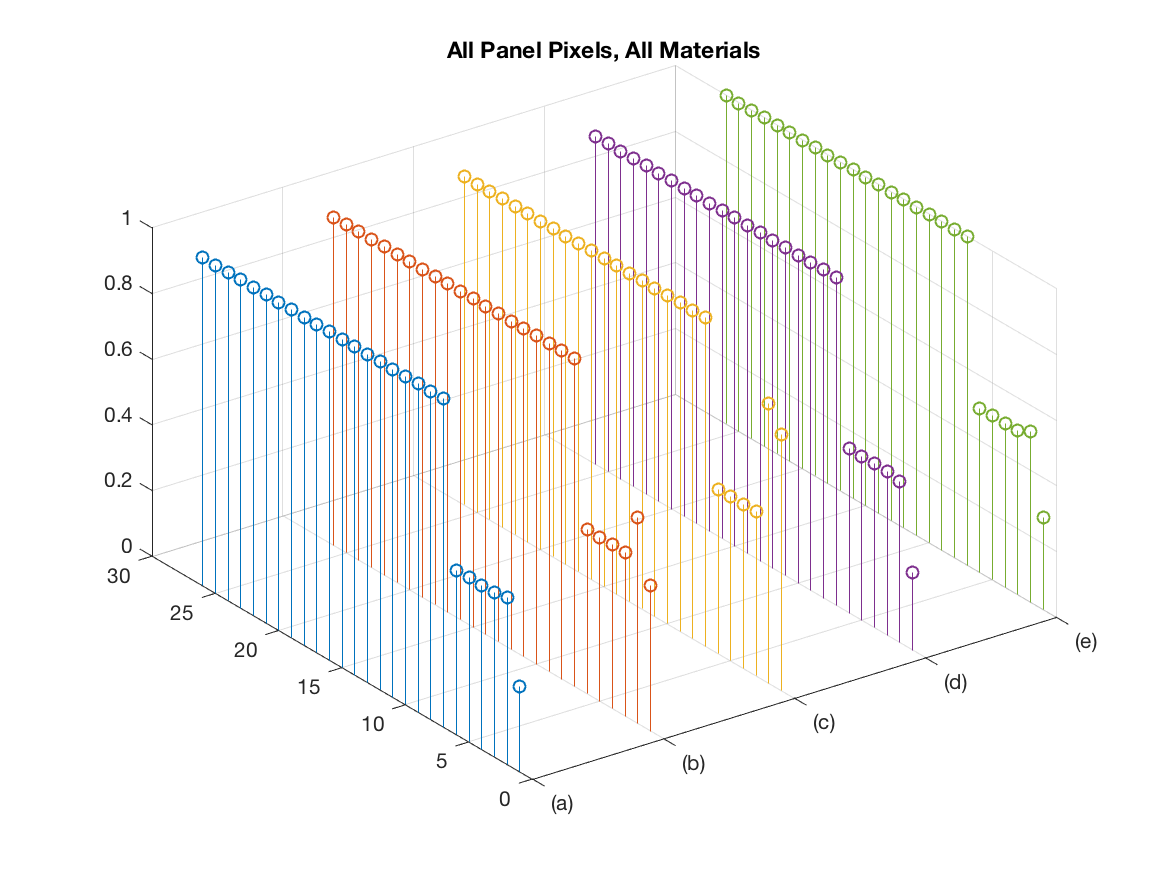
\includegraphics[width=3.5in]{mfcls_ti2_allmaterials.png}
    \caption{MFCLS, Augmented Active Set Method for TI2}
    \label{fig:mfcls_ti2}
\end{figure}

%fcls_te2_allmaterials.png
\begin{figure}[!h]
    \centering
    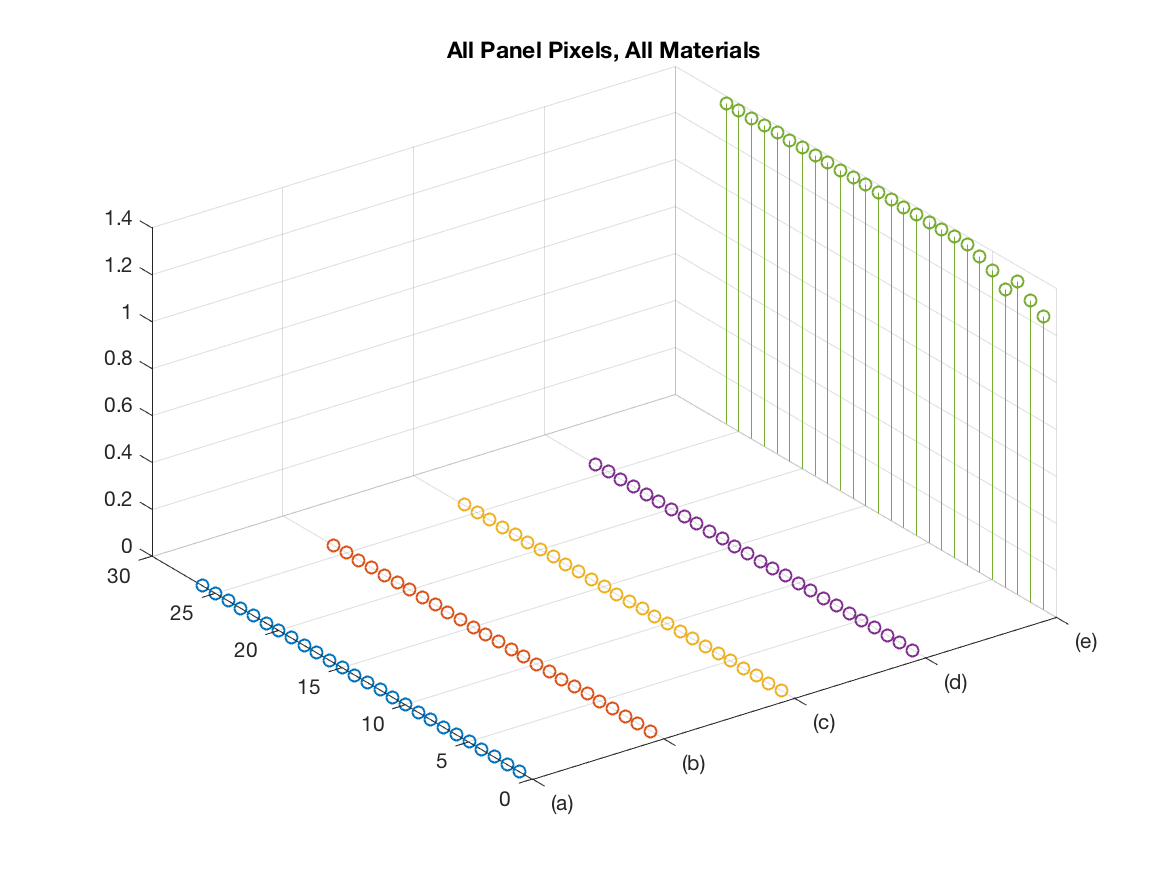
\includegraphics[width=3.5in]{fcls_te2_allmaterials.png}
    \caption{FCLS, Active Set Method for TE2}
    \label{fig:fcls_te2}
\end{figure}

%gfcls_te2_allmaterials.png
\begin{figure}[!h]
    \centering
    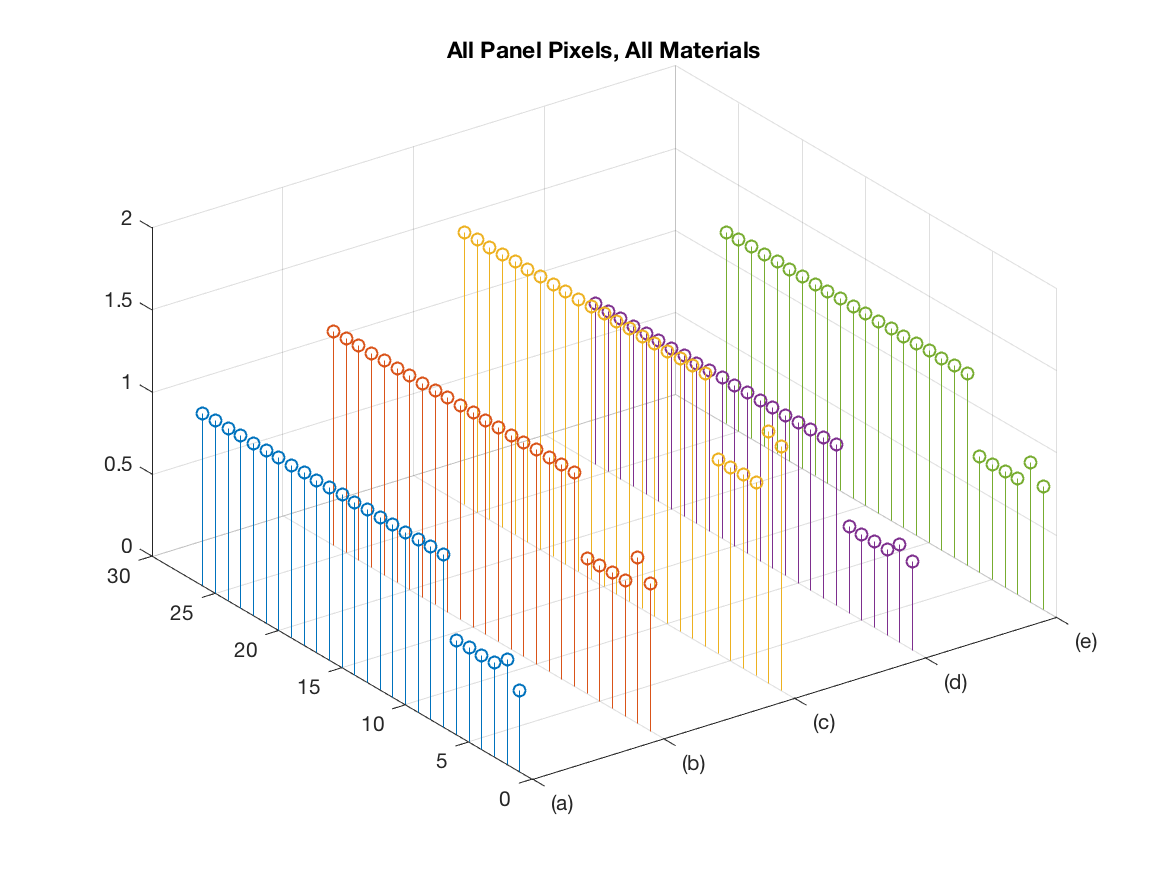
\includegraphics[width=3.5in]{gfcls_te2_allmaterials.png}
    \caption{FCLS, Geometric Volume Method for TE2}
    \label{fig:gfcls_te2}
\end{figure}

%osp_fcls_te2_allmaterials.png
\begin{figure}[!h]
    \centering
    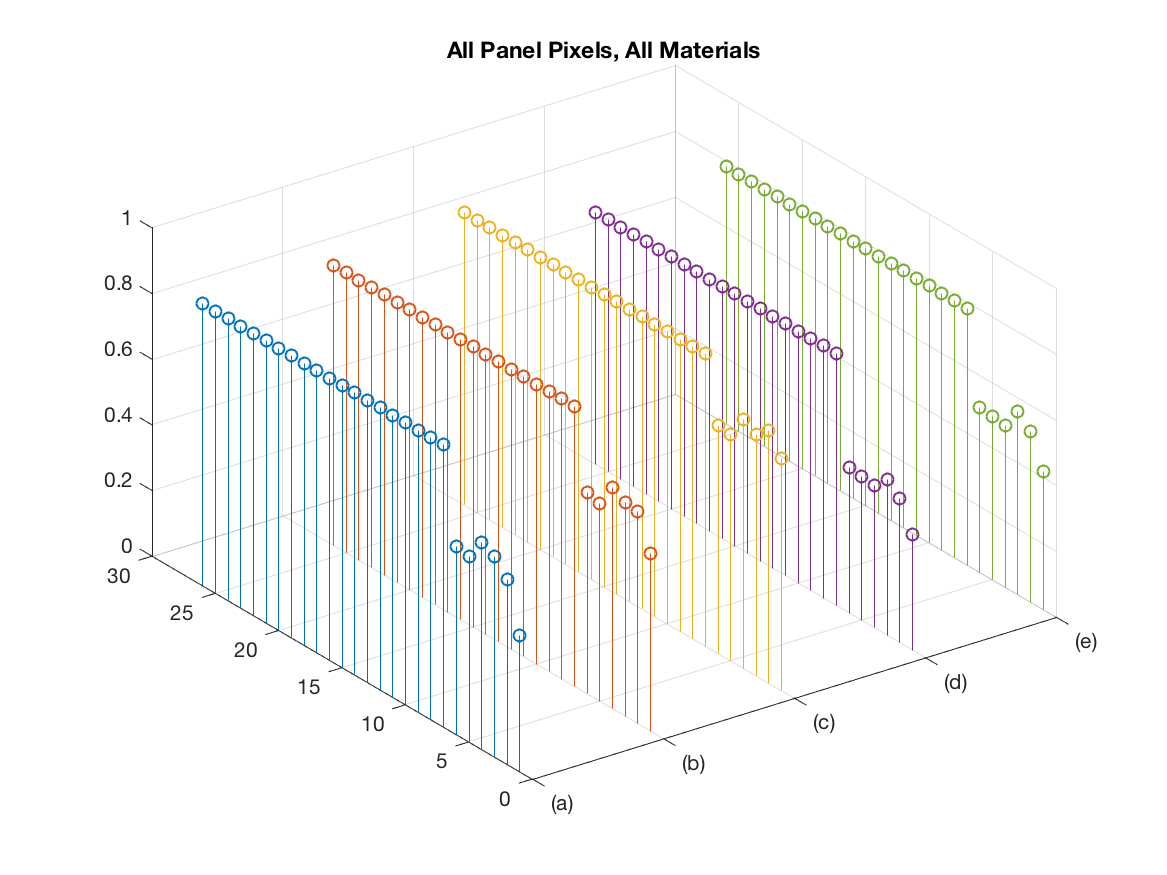
\includegraphics[width=3.5in]{osp_fcls_te2_allmaterials.png}
    \caption{FCLS, OSP Method for TE2}
    \label{fig:osp_fcls_te2}
\end{figure}

%mfcls2_te2_allmaterials.png
\begin{figure}[!h]
    \centering
    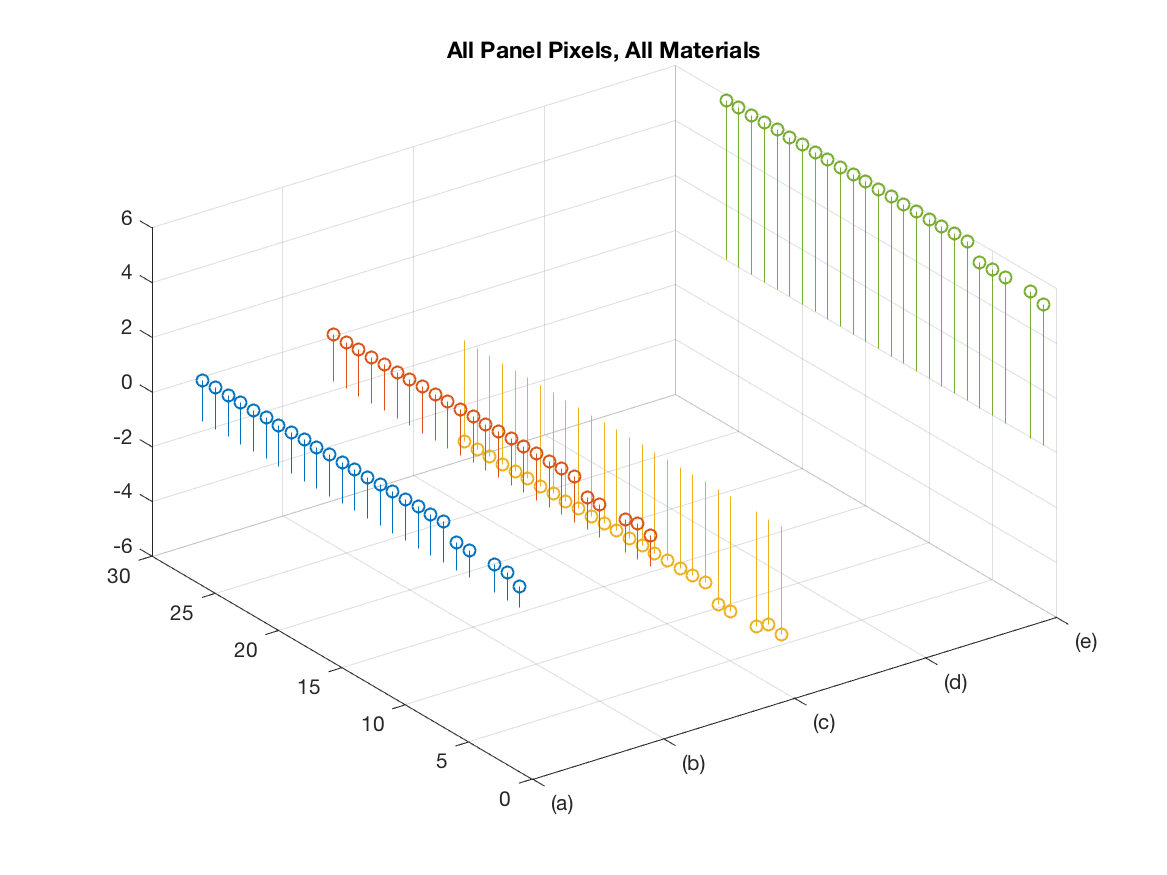
\includegraphics[width=3.5in]{mfcls2_te2_allmaterials.png}
    \caption{MFCLS, Lagrange Multiplier Method for TE2}
    \label{fig:mfcls2_te2}
\end{figure}

%mfcls_te2_allmaterials.png
\begin{figure}[!h]
    \centering
    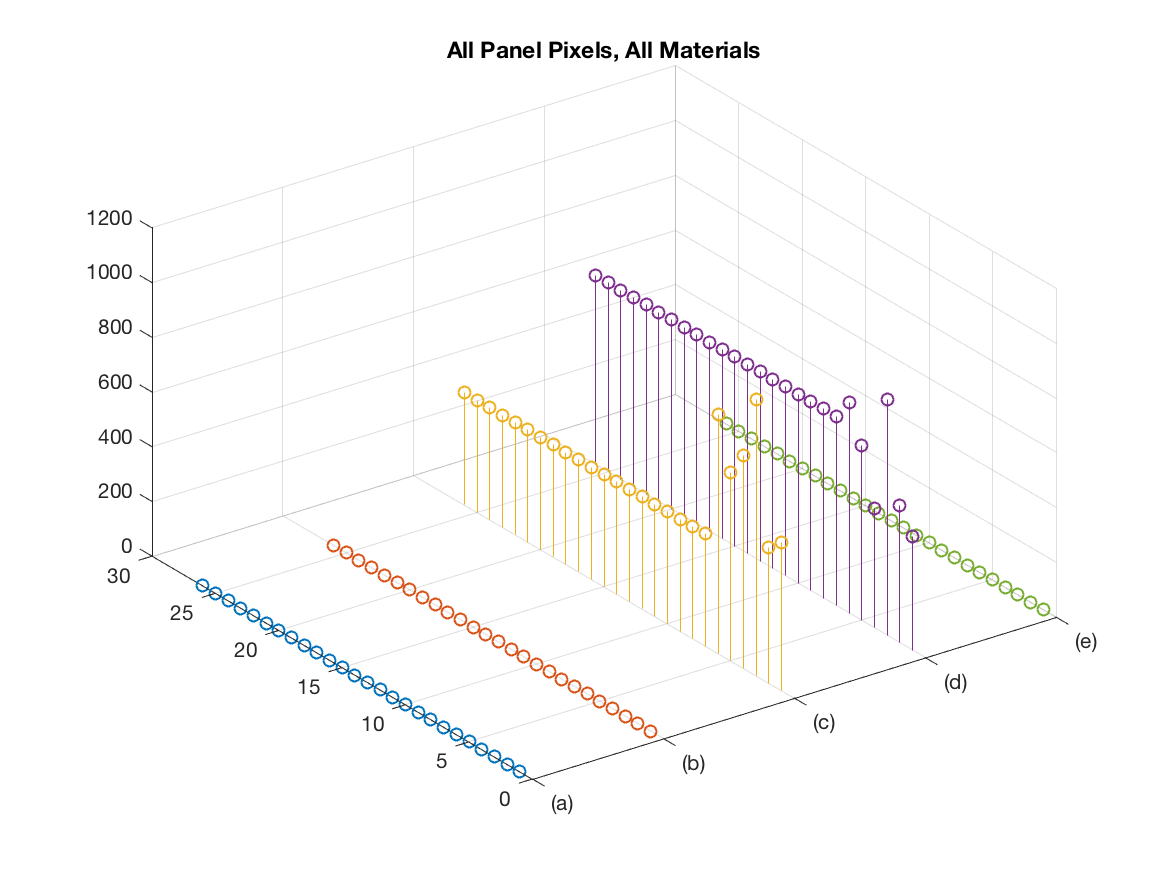
\includegraphics[width=3.5in]{mfcls_te2_allmaterials.png}
    \caption{MFCLS, Augmented Active Set Method for TE2}
    \label{fig:mfcls_te2}
\end{figure}

\onecolumn

%direct_ti2_nmf_endmembers.png
\begin{figure}[!t]
    \captionsetup[subfigure]{labelformat=empty}
    \begin{subfigure}[t]{0.5\textwidth}
    \centering
    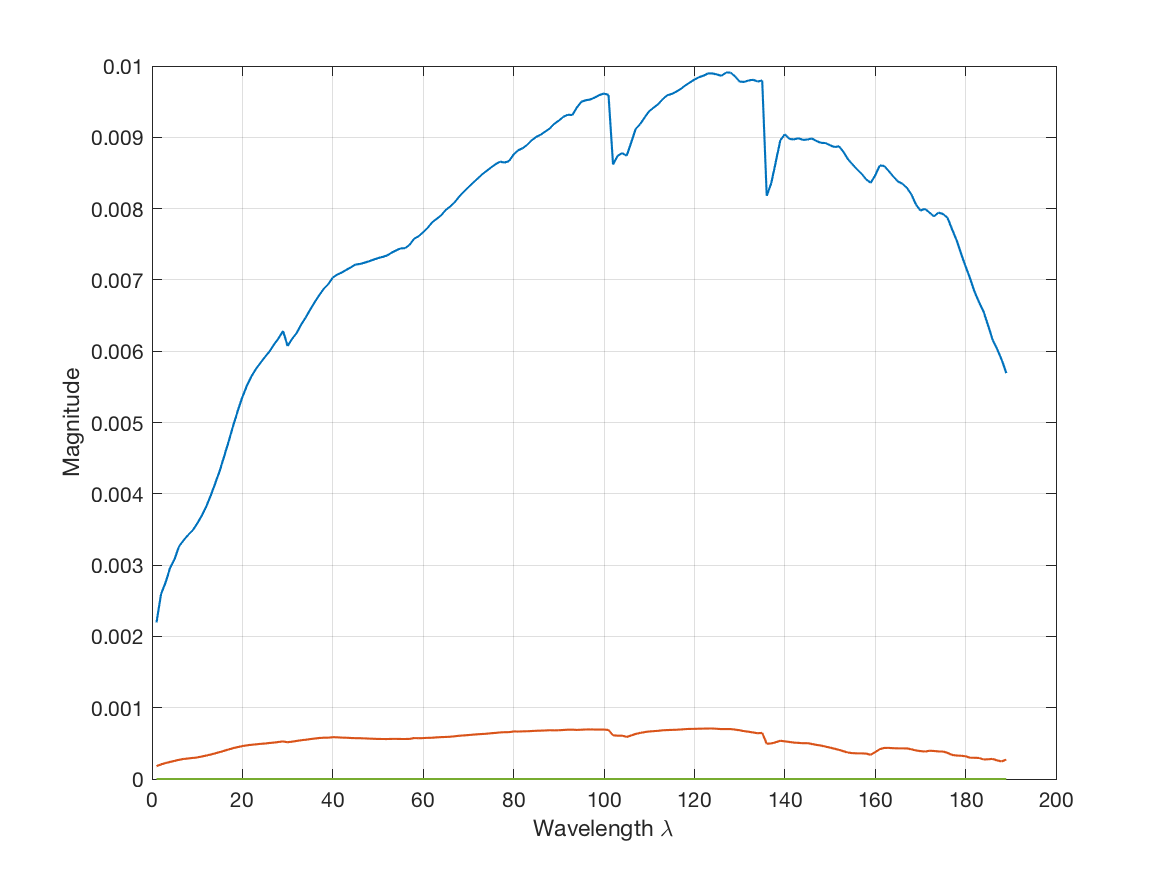
\includegraphics[width=3.5in]{direct_ti2_nmf_endmembers.png}
    \caption{Fig 14. Direct NMF TI2 Endmembers}
    \label{fig:direct_nmf_ti2_endmembers}
    \end{subfigure}
~
%direct_te2_nmf_endmembers.png
    \begin{subfigure}[t]{0.5\textwidth}
    \centering
    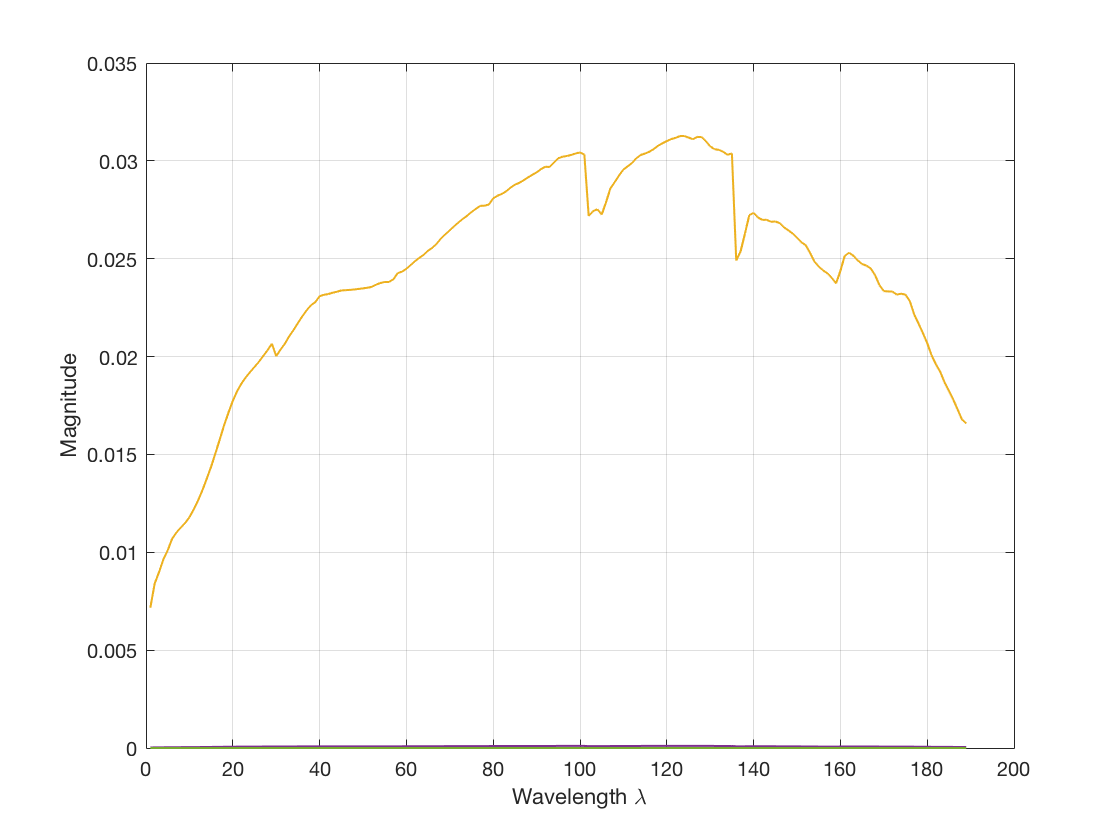
\includegraphics[width=3.5in]{direct_te2_nmf_endmembers.png}
    \caption{Fig 15. Direct NMF TE2 Endmembers}
    \label{fig:direct_nmf_te2_endmembers}
    \end{subfigure}

%direct_ti2_nmf_allmaterials.png
    \begin{subfigure}[b]{0.5\textwidth}
    \centering
    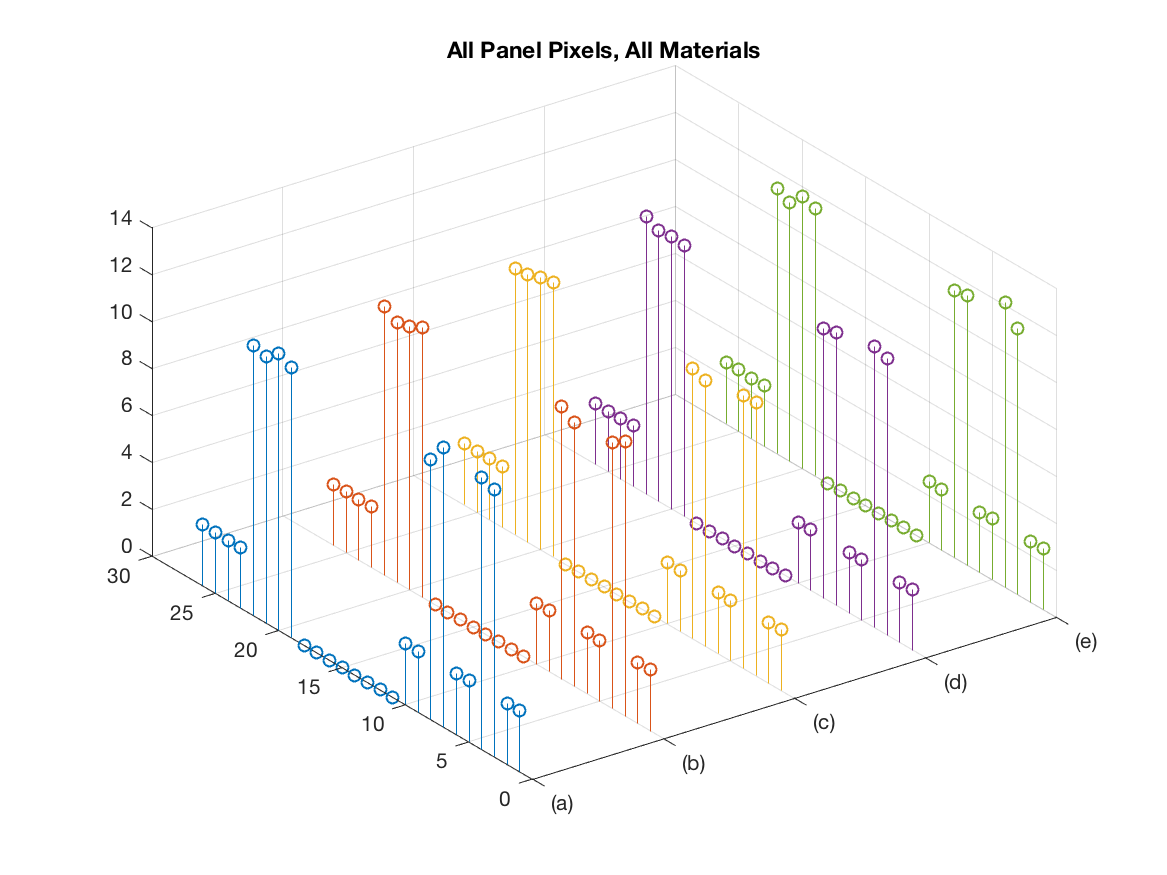
\includegraphics[width=3.5in]{direct_ti2_nmf_allmaterials.png}
    \caption{Fig 16. Direct NMF TI2 Abundance Fractions}
    \label{fig:direct_nmf_ti2_abundance}
    \end{subfigure}
~
%direct_te2_nmf_allmaterials.png
    \begin{subfigure}[b]{0.5\textwidth}
    \centering
    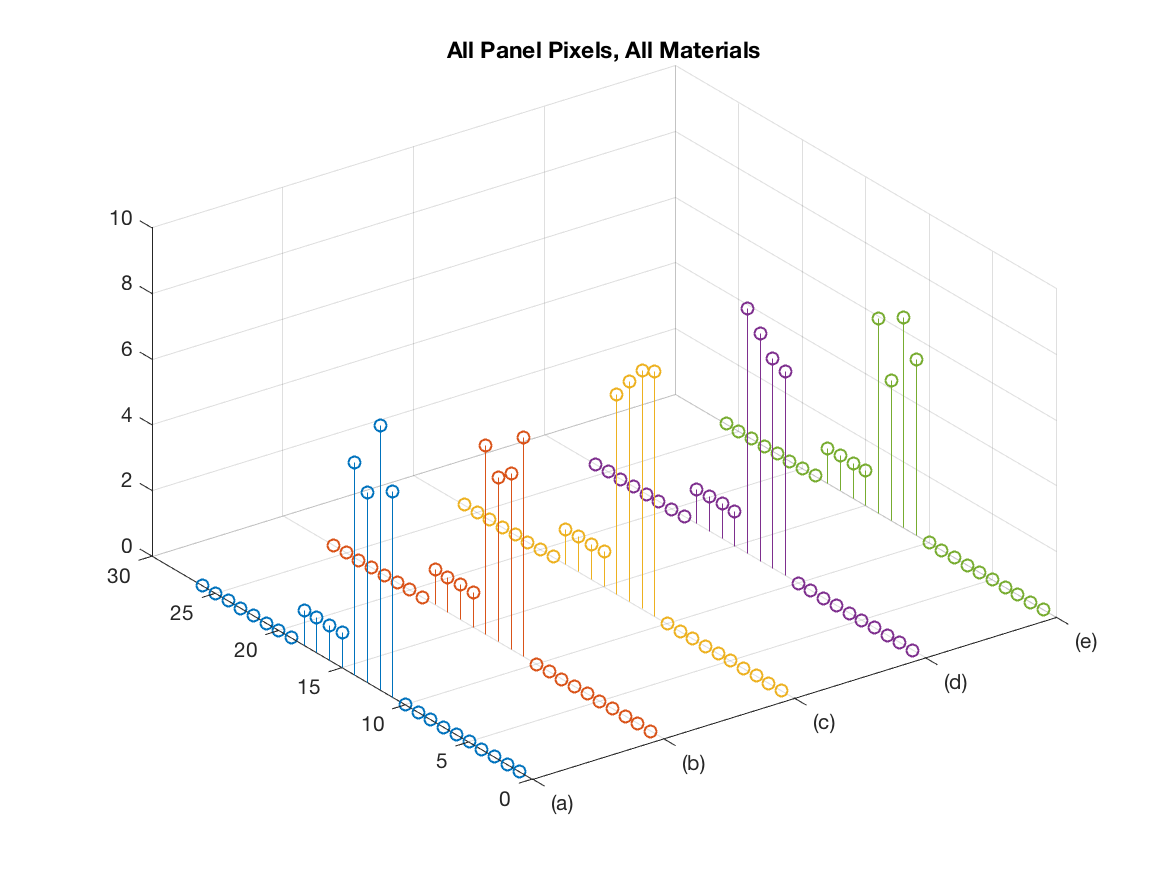
\includegraphics[width=3.5in]{direct_te2_nmf_allmaterials.png}
    \caption{Fig 17. Direct NMF TE2 Abundance Fractions}
    \label{fig:direct_nmf_te2_abundance}
    \end{subfigure}
\end{figure}

%nmf_endmembers_ti2_70.png
\begin{figure}[!t]
    \captionsetup[subfigure]{labelformat=empty}
    \begin{subfigure}[t]{0.5\textwidth}
    \centering
    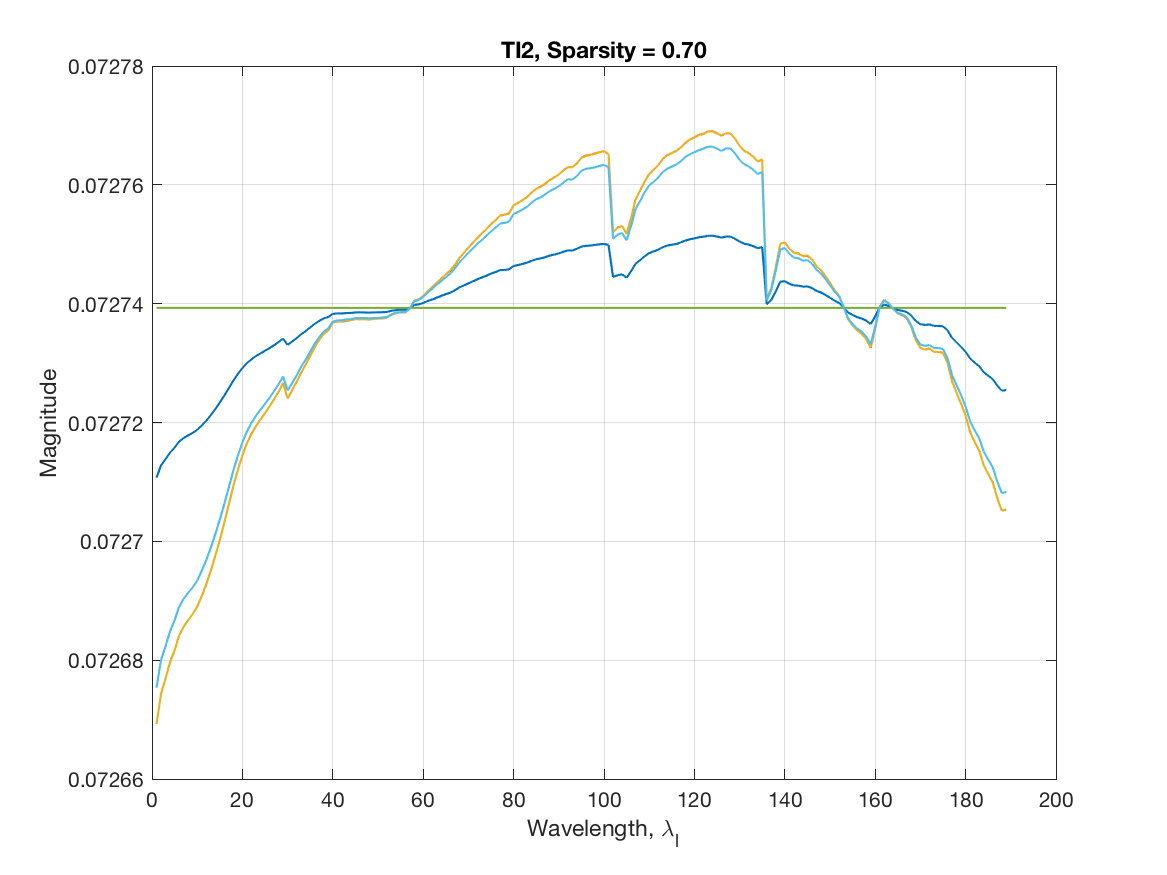
\includegraphics[width=3.5in]{nmf_endmembers_ti2_70.png}
    \caption{Fig. 18 Endmembers for Sparse NMF TI2 sparsity = 0.70}
    \label{fig:nmf_end_ti2_70}
    \end{subfigure}
~
%nmf_endmembers_te2_70.png
    \begin{subfigure}[t]{0.5\textwidth}
    \centering
    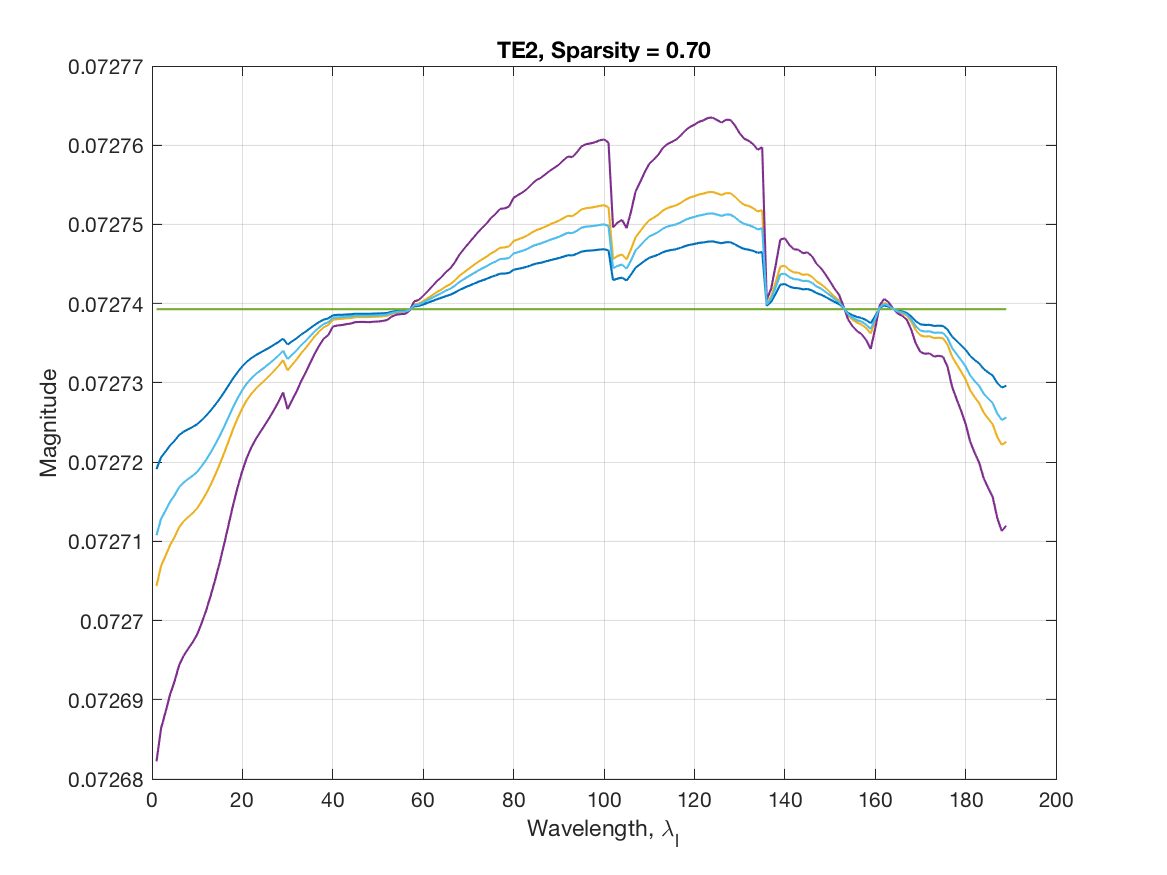
\includegraphics[width=3.5in]{nmf_endmembers_te2_70.png}
    \caption{Fig 19. Endmembers for Sparse NMF TE2 sparsity = 0.70}
    \label{fig:nmf_end_te2_70}
    \end{subfigure}

%nmf_abundance_ti2_70_allmaterials.png
    \begin{subfigure}[b]{0.5\textwidth}
    \centering
    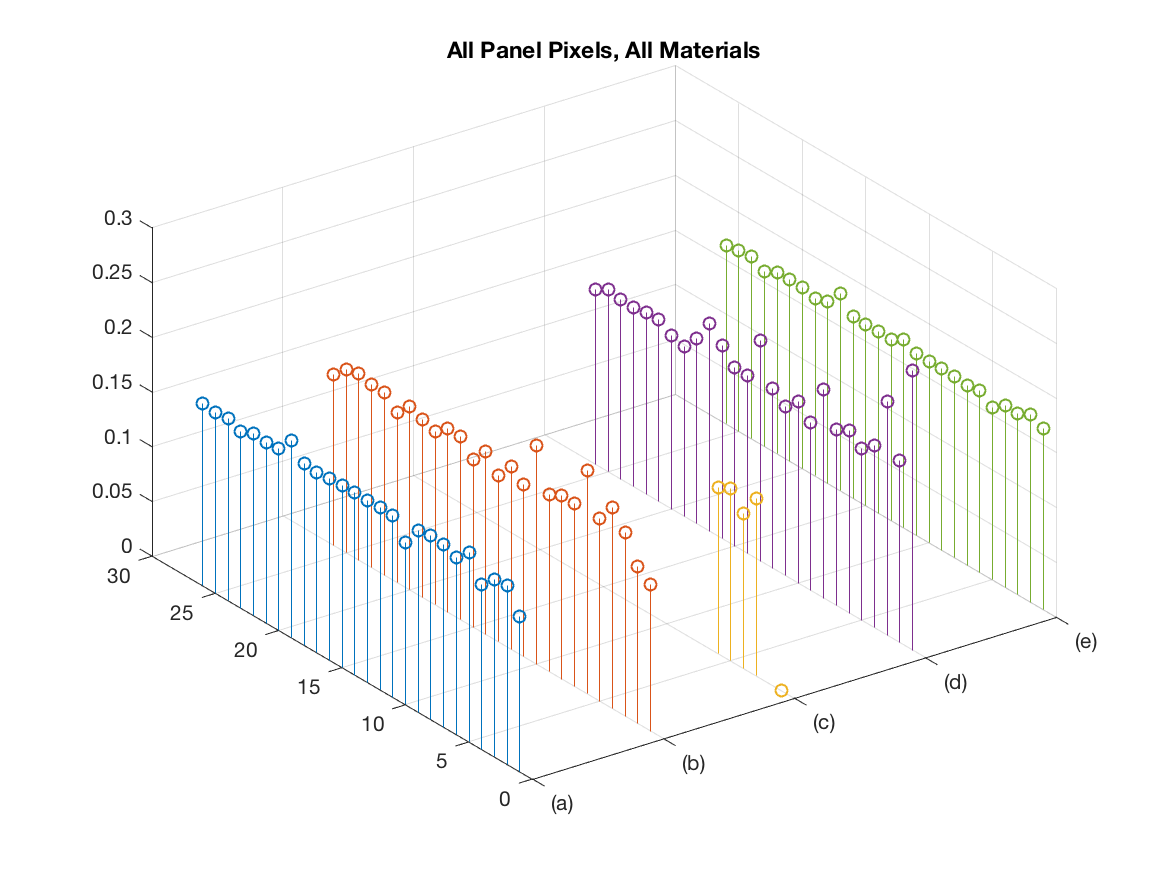
\includegraphics[width=3.5in]{nmf_abundance_ti2_70_allmaterials.png}
    \caption{Fig 20. Abundance Fractions for TI2 and sparsity = 0.70}
    \label{fig:nmf_abund_ti2_70}
    \end{subfigure}
~
%nmf_abundance_te2_70_allmaterials.png
    \begin{subfigure}[b]{0.5\textwidth}
    \centering
    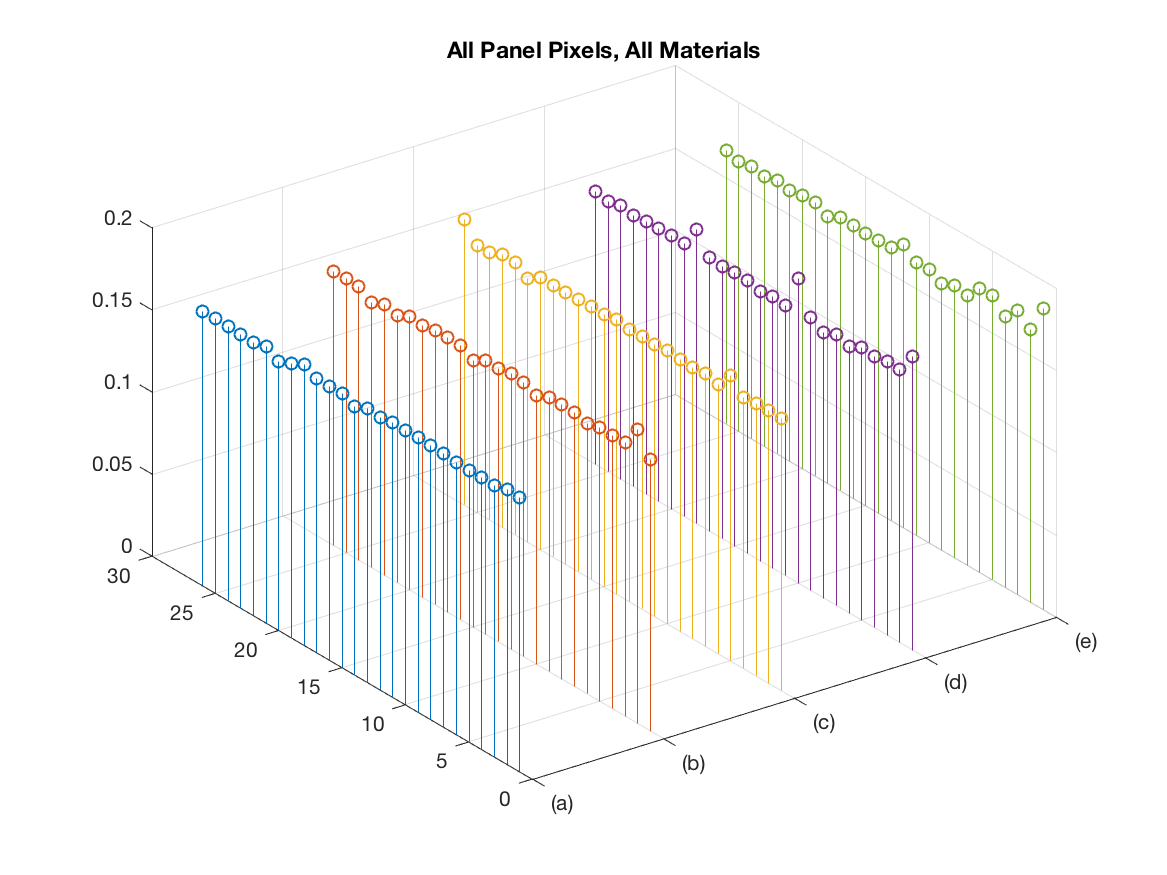
\includegraphics[width=3.5in]{nmf_abundance_te2_70_allmaterials.png}
    \caption{Fig 21. Abundance Fractions for TE2 and sparsity = 0.70}
    \label{fig:nmf_abund_te2_70}
    \end{subfigure}
\end{figure}

\twocolumn

% references section
% bibliography generated by BibTeX as a .bbl file
\nocite{*}
\bibliographystyle{IEEEtran}
\bibliography{report}

\begin{IEEEbiography}{Bernard Lampe}
 (S'09) became a IEEE Student Member (S) in 2009 and received his bachelors of computer science degree from The University of Michigan in Ann Arbor, Michigan, USA in 2009. He received his masters in electrical engineering from the University of Maryland Baltimore County (UMBC) in 2016. His interests are computer vision, image processing and compressive sensing. He is currently pursuing his doctorate in electoral engineering at UMBC.
\end{IEEEbiography}

\end{document}

